
\begin{figure}[ht]
    \centering
    \vspace{-.75em}
    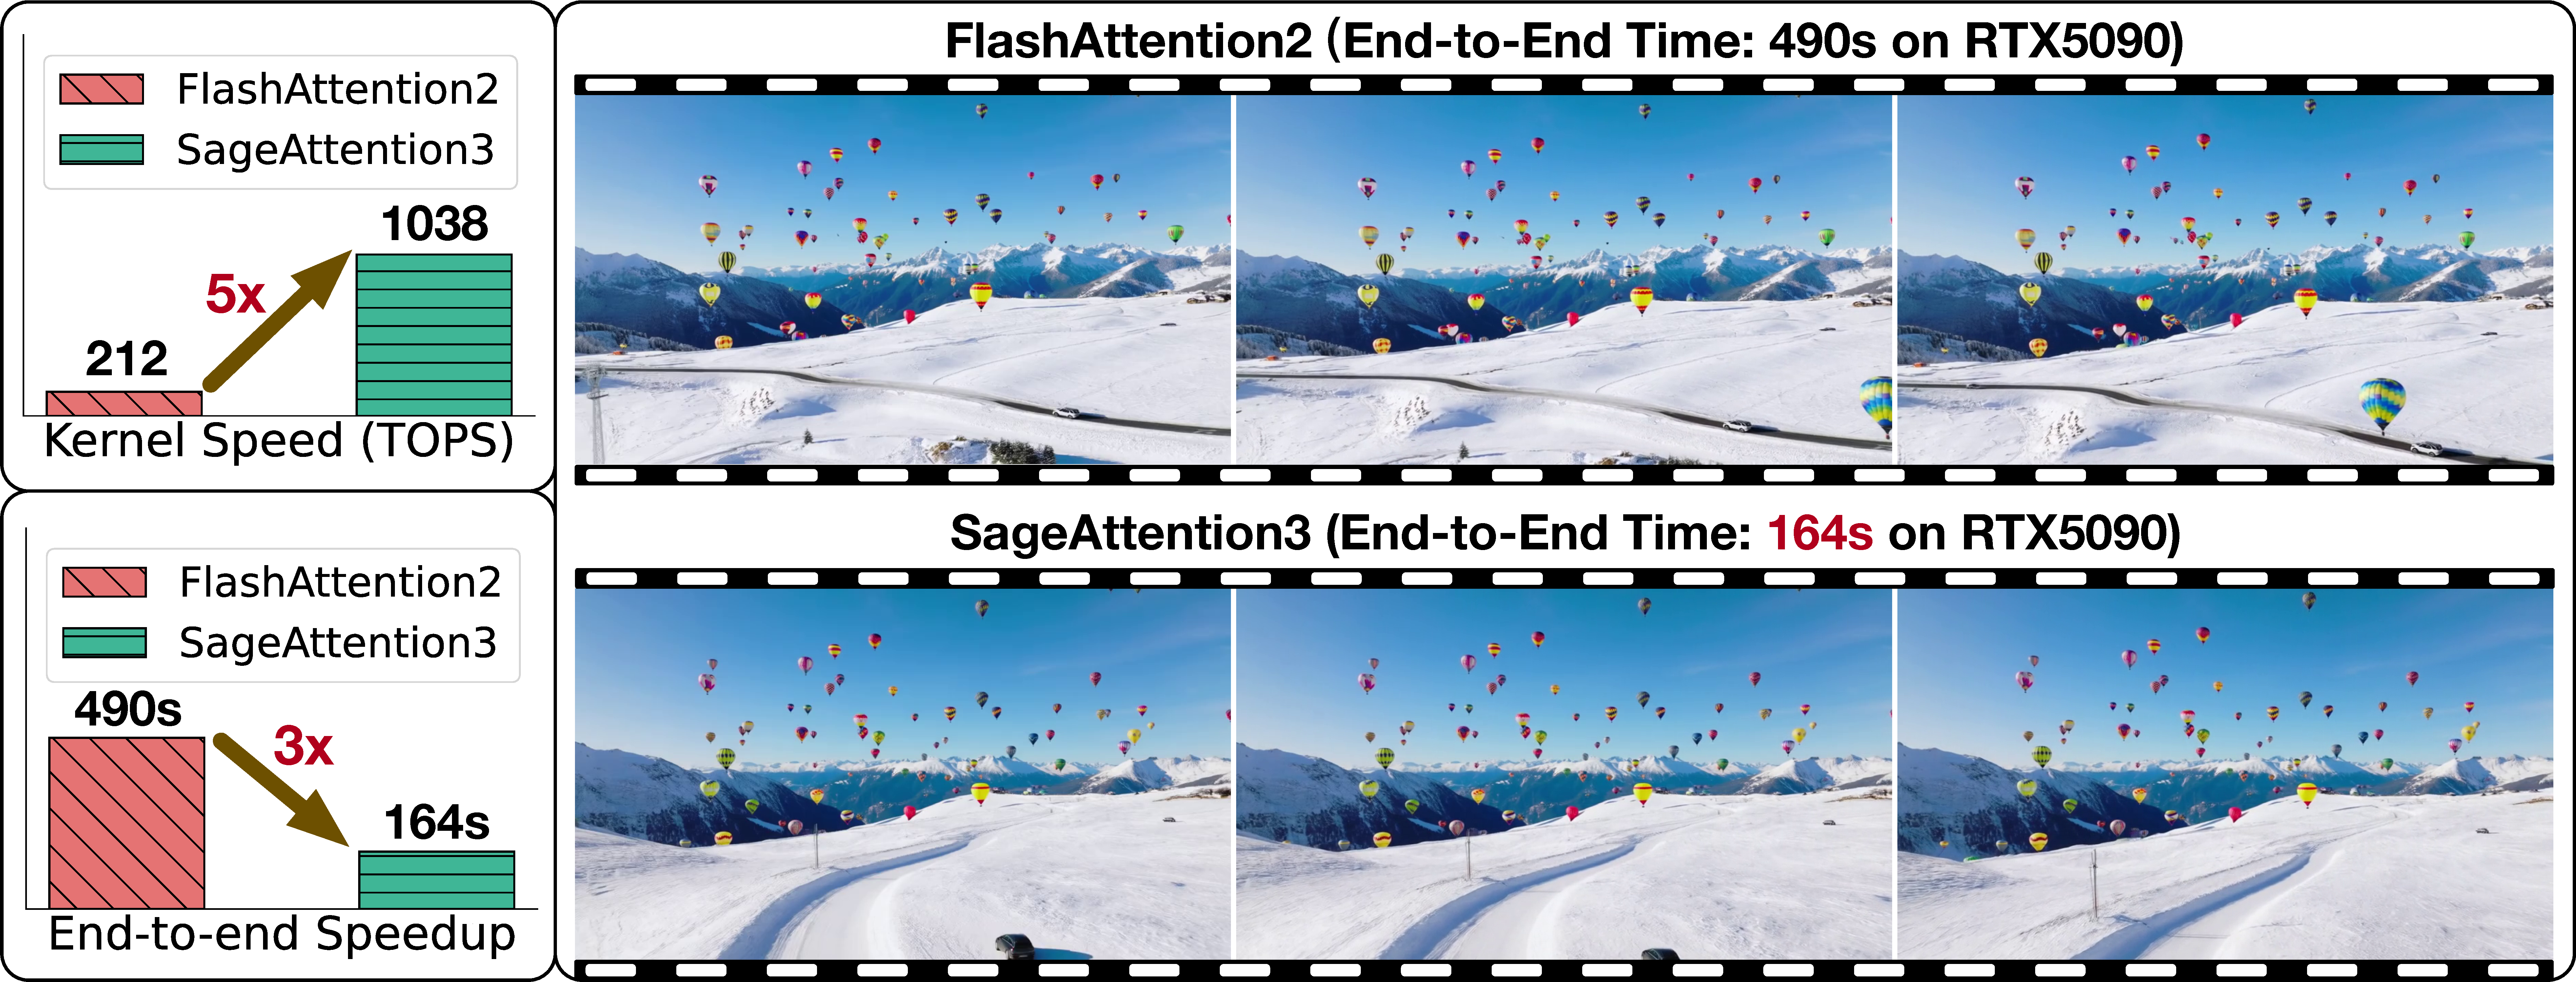
\includegraphics[width=.91\columnwidth]{src/figs/cover.pdf} 
    % \vspace{-1em}
    \caption{The upper left figure shows the kernel speedup on \texttt{RTX5090}. The other two figures show the end-to-end inference speedup of generating a video using \texttt{HunyuanVideo} on \texttt{RTX5090}. Note that FlashAttention3 can only run on Hopper GPUs, so FlashAttention2 is already the fastest on \texttt{RTX5090}.}
    \vspace{-1em}
    \label{fig:cover} 
\end{figure}


\section{Introduction}
\textbf{Motivation}. 
The efficiency of attention is critical for generation models, especially given their quadratic time complexity with longer sequences~\citep{vaswani2017attention,zhangsurvey}. Quantization offers an effective way to accelerate inference by utilizing low-bit Tensor Cores in GPUs~\citep{2024sageattention,zhang2024sageattention2,zhang2025turbodiffusion,chen2020statistical}. The new \texttt{FP4} Tensor Cores in Blackwell GPUs deliver significantly faster performance compared to \texttt{FP16}~\citep{whitepaper5090}. We want to propose a novel \texttt{FP4} attention implementation that provides plug-and-play compatibility for inference acceleration. Beyond inference, training efficiency is equally important. However, no prior work has explored low-bit attention for training large models. To address this gap, we design a trainable \texttt{8-bit} attention to explore its feasibility in training tasks.

To the best of our knowledge, we are the \underline{first work} that designs \texttt{FP4} attention for inference and the \underline{first work} to explore the feasibility of low-bit attention for training large models.

\textbf{Challenges.} 
There are two primary obstacles for \texttt{FP4} attention and one key difficulty for \texttt{8-bit} trainable attention. First, \textbf{(C1)} \texttt{FP4} quantization suffers from severe value limitations (only 15 representable values), making both per-tensor and per-token quantization approaches inadequate for preserving model accuracy. Second, \textbf{(C2)} The attention map \( P \) consists primarily of small values in the range \([0, 1]\). When directly quantized to \texttt{FP4}, these values force the scaling factors into an extremely narrow dynamic range. However, hardware requires the quantization factors to be in \texttt{FP8} data type. This leads to significant accuracy loss when presenting these scale factors in \texttt{FP8}. 
Third, \textbf{(C3)} When employing \texttt{8-bit} attention during training, we find that the attention map gradients are particularly vulnerable to quantization errors, resulting in accumulated errors in the input gradients.

\textbf{Our Method.} To address \textbf{(C1)}, we propose to use \texttt{FP4} microscaling quantization for the two matrix multiplications in attention, i.e., $QK^\top$ and $PV$. 
By constraining the quantization group size to 1x16 (instead of per-tensor or per-channel), our method effectively contains outlier effects within each block while improving \texttt{FP4} quantization accuracy.
To overcome \textbf{(C2)}, we propose a two-level quantization method for $P$ to fully utilize the presentative range of the \texttt{FP8} scaling factor, enhancing the quantization accuracy of $P$. Specifically, this approach first normalizes each token's range to $\mathsf{[0, 448 \times 6]}$ through per-token quantization, then applies \texttt{FP4} microscaling quantization for enhanced precision.
To address \textbf{(C3)}, we identify the most accuracy-sensitive matrix multiplication among the five in backpropagation and maintain its accuracy in \texttt{FP16}.

\textbf{Result.} Our \texttt{FP4} attention, named \our, could achieve \textbf{1038} \texttt{TOPS} on \texttt{RTX5090}, which is a \textbf{5}$\times$ speedup than FlashAttention. Furthermore, we demonstrate that \texttt{8-bit} trainable attention, named \texttt{SageBwd}, could achieve lossless performance when fine-tuning base models for instruction-following tasks, but is not suitable for pretraining tasks. 

\textbf{Contribution.} Our work makes the following key contributions:

\textbf{(1)} We design the first \texttt{FP4} attention to accelerate inference, achieving \textbf{1000+} \texttt{TOPS} on \texttt{RTX5090}.

\textbf{(2)} We propose the first trainable low-bit attention, enabling accelerated training with lossless fine-tuning performance, while revealing key insights for low-bit attention in training.

\begin{figure}[ht]
    \centering
    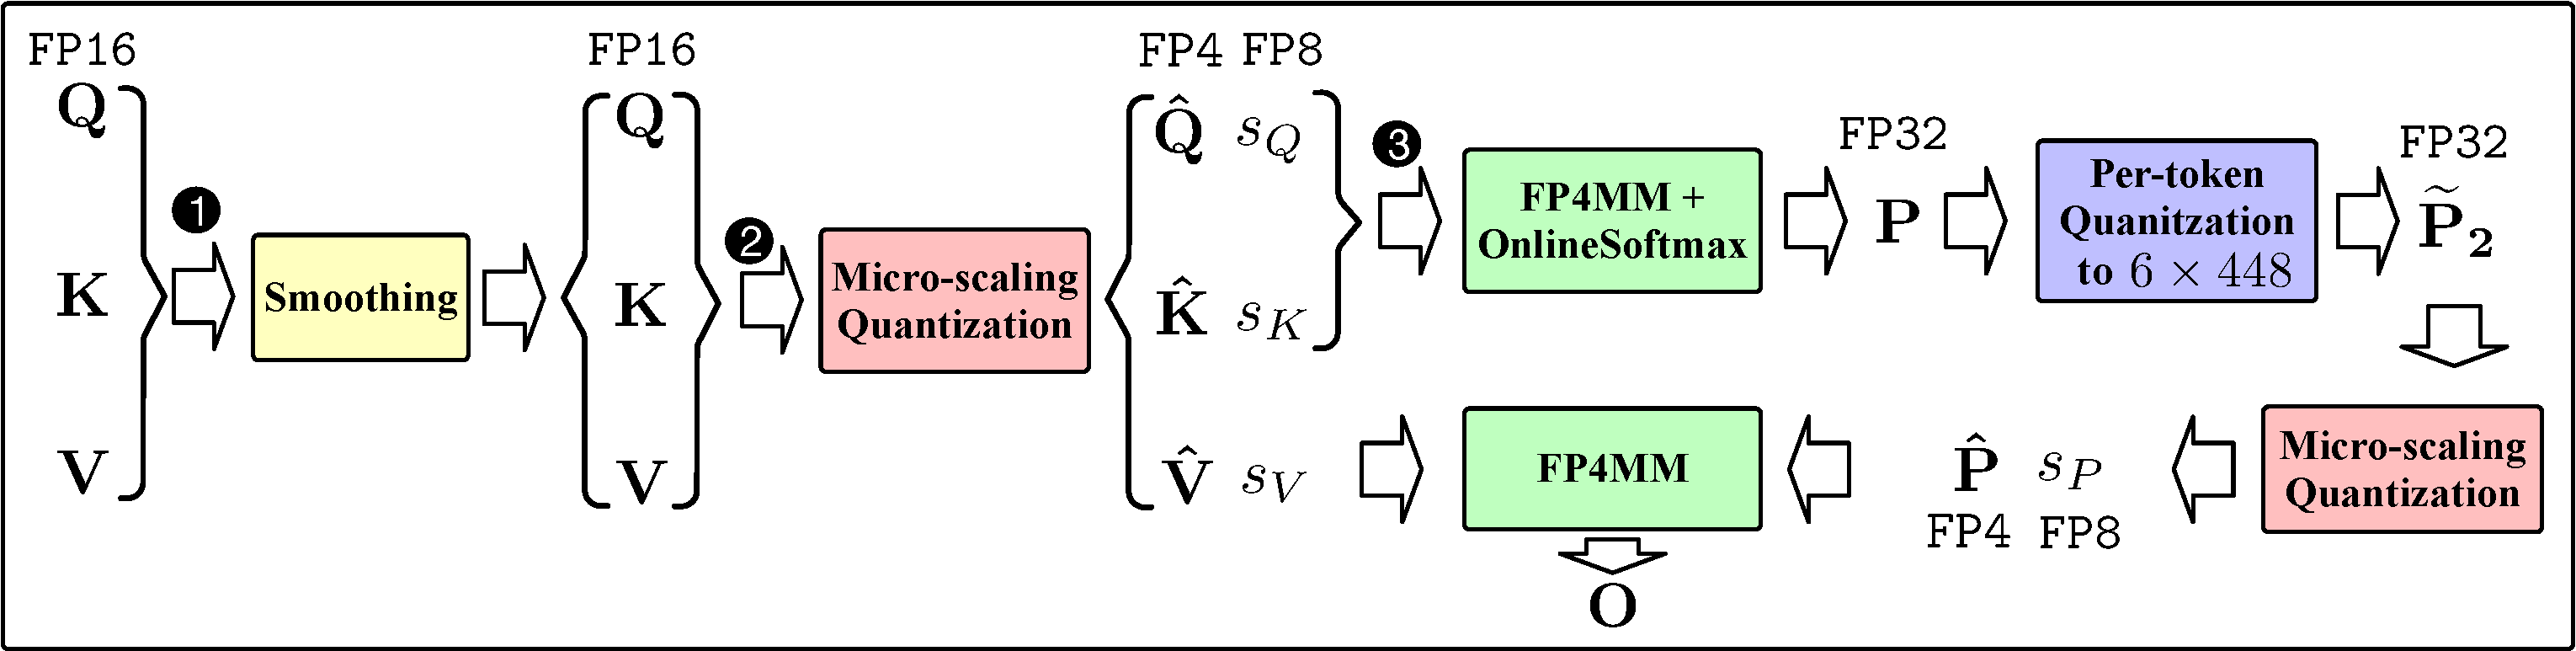
\includegraphics[width=\columnwidth]{src/figs/alg_overview.pdf} 
    \caption{Workflow of microscaling \texttt{FP4} attention.}
    \label{fig:workflow}
\end{figure}

\section{Preliminary}  \label{sec:preliminary}
\textbf{FlashAttention.} The attention computation contains two matrix multiplications and one softmax calculation: $S = QK^\top, P = \texttt{Softmax}(S), O = PV$. The $Q, K, V$ are in the shape of $N \times D$, where $N$ means the sequence length and $D$ means the dimension of an attention head. $P, S$ are in the shape of $N \times N$. FlashAttention divides $Q$ to blocks $\{Q_i\}$ in the shape of $B_q \times D$, and divides $K, V$ to $\{K_i\}, \{V_i\}$ in the shape of $B_{kv} \times D$. Then it uses online softmax to avoid the large memory IO for $S$ and $P$: $S_{ij} = Q_iK_j^\top, P_{ij} = \texttt{OnlineSoftmax}(S_{ij}), O_{ij} = P_{ij}V_{j}$.

\textbf{Notation.} For simplicity, we omit subscripts and use $\vQ, \vK, \vV, \vS, \vP, \vO$ to denote the matrix blocks in FlashAttention, while retaining full subscript notation in Algorithm~\ref{alg:sage3_fwd},~\ref{alg:int8_train_fwd}, and~\ref{alg:int8_train_bwd}.


\textbf{Quantization.} Quantization is used to accelerate Matmul by converting two matrices from high-bit to low-bit with scale factors. Take \texttt{INT8} quantization for Matmul $AB$ as an example, where $A$ and $B$ are in \texttt{FP16} data type. It can be formulated: $s_A = \max(|A|)/127, ~\hat A =  \lceil A / s_A \rfloor$, $s_B = \max(|B|)/127, ~\hat B = \lceil B / s_B \rfloor$, where $\hat A, \hat B$ are in \texttt{INT8} and the others are in \texttt{FP32}. Then, $AB \approx \hat A \hat B \times s_A \times s_B$, which can be accelerated by the \texttt{INT8} Tensor Core. The granularity of quantization is determined by the dimensions reduced by the $\max$ operation. For example, in \textit{per-token quantization}, the $\max$ is computed along each row of a matrix. In \textit{per-block quantization}, the $\max$ is computed on a block of a matrix, which in our paper means a FlashAttention block.



% \textbf{Quantization:}~   s_{ij} = \max(|X|)/6, ~~~   \hat X_{ij} =   \lceil X_{ij} / s_{ij} \rfloor,  \\
% \textbf{Dequantization:}~ [X_{ij}' = \phi^{-1}(\hat X_{ij}, s_{ij})]:~ X_{ij}' = s_{ij} \times \hat X_{ij}
% \label{equ:microscaling} 